\documentclass[10pt]{beamer}

%%%%% ===== 设置主题 *****
\usetheme{Berlin}
% 可供选择的主题参见 beameruserguide.pdf
% 无导航条的主题: Bergen, Boadilla, Madrid, CambridgeUS,
%                 GoettingenAnnArbor,Pittsburgh, Rochester;
% 有树形导航条的主题: Antibes, JuanLesPins, Montpellier;
% 有目录竖条的主题: Berkeley, PaloAlto, Goettingen, Marburg, Hannover;
% 有圆点导航条的主题: Berlin, Ilmenau, Dresden, Darmstadt, Frankfurt, Singapore, Szeged;
% 有节与小节导航条的主题: Copenhagen, Luebeck, Warsaw

\useinnertheme{circles}
\useoutertheme{infolines}
\usefonttheme[onlymath]{serif}
\setbeamertemplate{navigation symbols}{} % remove the navigation
\setbeamersize{text margin left=0.8cm, text margin right=0.8cm}
\setbeamerfont{frametitle}{size=\large}
\setbeamerfont{footline}{family=\ttfamily}\setbeamertemplate{caption}[numbered]
%%%%% ===== 宏包 *****
\usepackage{amsmath,amssymb,amsfonts,ragged2e}
\usepackage{graphicx,xcolor}
\usepackage{hyperref}
\usepackage{bm}
\usepackage{amsthm}
\usepackage{ulem}
\usepackage{multirow}
\usepackage{tcolorbox}
% \usepackage{xeCJK}
% \usepackage{algorithmicx,algorithm}
\usepackage[linesnumbered,ruled,vlined]{algorithm2e}
\SetKwInOut{KwIn}{Init}
\usepackage[backend=bibtex,style=numeric,sorting=none]{biblatex}
\addbibresource{reference.bib}
\setbeamerfont{footnote}{size=\tiny}
\renewcommand{\baselinestretch}{1.1}
\usepackage[UTF8]{ctex}
% \setCJKfamilyfont{myfont}{STSong}
% \newcommand{\MyFont}{\CJKfamily{myfont}}
%%%%% ===== 自定义命令 *****
\newcommand{\myem}[1]{\textcolor{blue}{#1}}
\renewcommand{\today}{\number\year 年\number\month 月\number\day 日}
\renewcommand{\figurename}{图}
\renewcommand{\tablename}{表}
\setbeamerfont{caption}{size=\footnotesize}
%\newtheorem{theorem}{Theorem}

\begin{document}
\justifying
\title[求解混合整数双层线性规划问题的分支定界算法研究]%
{求解混合整数双层线性规划问题的分支定界算法研究}

\author[杜洪博]%
{报告人: 杜洪博\\
导\quad 师: 寇彩霞\rule[0pt]{0pt}{20pt}\\}

\institute[BUPT]{\textcolor[rgb]{0.0,0.0,0.10}%
{\small\ttfamily 北京邮电大学\ 理学院\\[10pt]}}

\date{\today}

% ===== title page ====================================
\begin{frame}[plain]
	\titlepage
\end{frame}

\begin{frame}
	\frametitle{目录}
	\tableofcontents[hideallsubsections] %[pausesections]
\end{frame}

\AtBeginSection[] % Do nothing for \section*
{ \begin{frame}<beamer> %\frametitle{Outline}
		\tableofcontents[currentsection,hideallsubsections]%,currentsubsection]
	\end{frame}
}

%===== Main part start here ==========================
% 双层规划问题介绍
% 问题背景
% 混合整数双层规划问题的求解算法
% 数值实验
% 未来工作安排

\section{双层规划问题}

\begin{frame}
	\frametitle{双层规划问题简介\footfullcite{sinha_review_2018}}
	双层规划问题可以表示为如下形式: 
	\begin{equation}
		\begin{aligned}
			\min_{x,y}& F(x,y)  \\
			&G(x,y)\leq0 \\
			&y\in\arg\operatorname*{min}_{y^{\prime}}\{f(x,y^{\prime}):g(x,y^{\prime})\leq0\},
		\end{aligned}
	\end{equation}
	\begin{itemize}
		\item $x$为上层(Upper/Leader)变量;
		\item $y$为下层(Lower/Follower)变量;
		\item $F(x,y)$和$f(x,y)$分别为上层和下层的目标函数;
		\item $G(x,y)$和$g(x,y)$分别为上层和下层的约束条件.
	\end{itemize}
\end{frame}

\begin{frame}
	\frametitle{双层规划问题简介}
	\begin{figure}
		\centering
		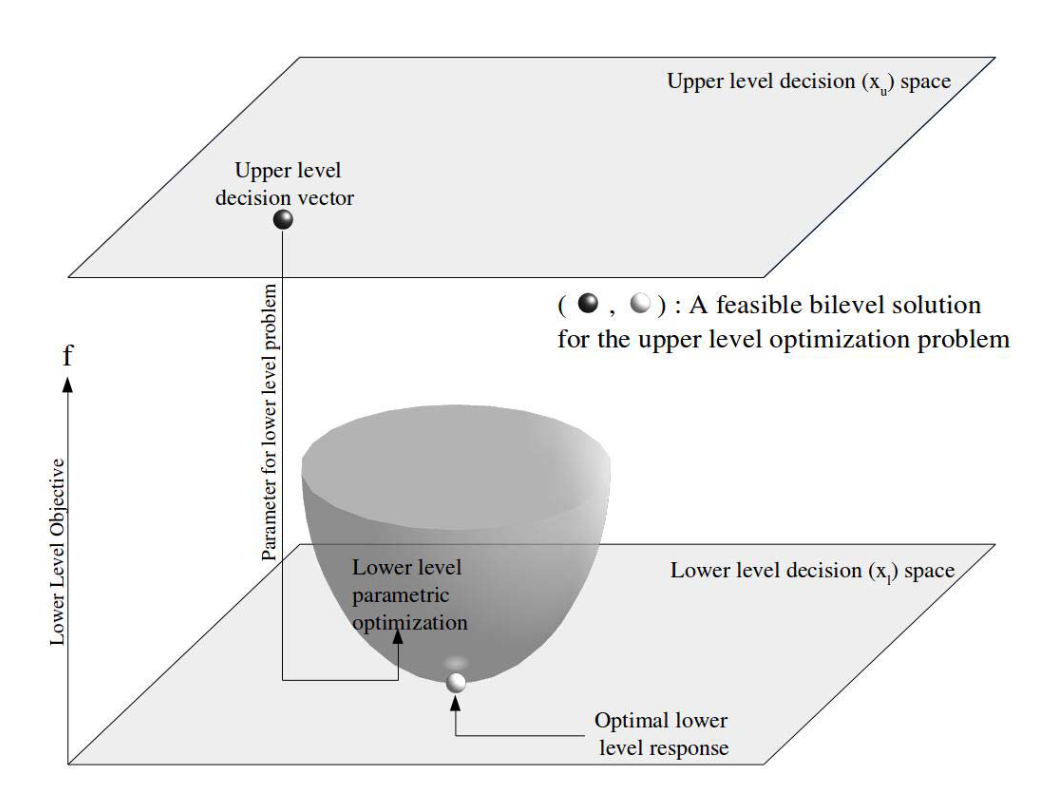
\includegraphics[width=0.7\textwidth]{pic/双层问题示意图.png}
		\caption{双层规划问题示意图}
	\end{figure}
\end{frame}

\section{问题背景}

\begin{frame}
	\frametitle{问题背景} 
	在多能互补电力系统优化问题中需要同时考虑系统经济性和供电稳定性,为了刻画该问题,可以将其建模为混合整数双层规划问题。
	\begin{figure}
		\centering
		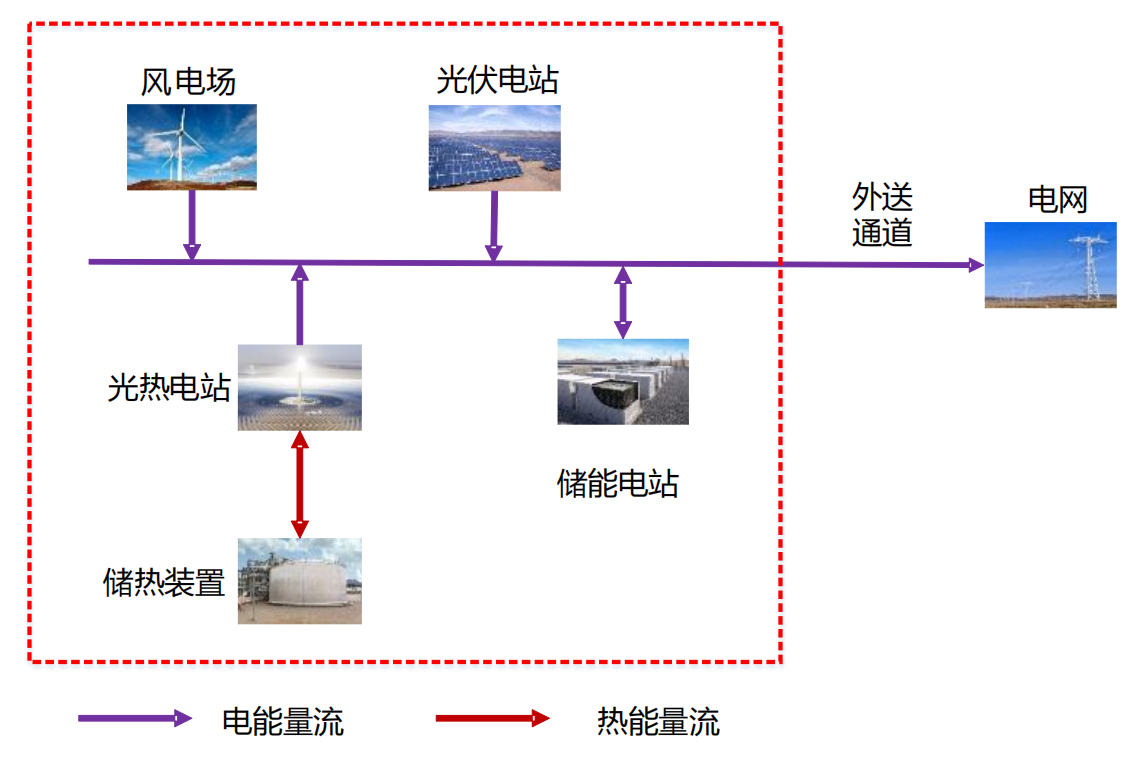
\includegraphics[width=0.65\textwidth]{pic/系统结构示意图.png}
		\caption{系统示意图}
	\end{figure}
\end{frame}

\section{一种混合整数双层规划问题求解算法} 

\begin{frame}
	Fischetti, M., Ljubić, I., Monaci, M. et al. On the use of intersection cuts for bilevel optimization. Math. Program. 172, 77–103 (2018). 
\end{frame}

\begin{frame}
	\frametitle{MIBLP}
	混合整数双层线性规划问题可以表示为如下形式:
	\begin{equation}
		\begin{aligned}
			\min_{x,y}~~&c_{x}^{T}x+c_{y}^{T}y \\
			&G_xx+G_yy \leq q  \\
			&x_{j}\mathrm{~integer}, \forall j\in J_{x}  \\
			&y\in\operatorname{arg}\operatorname*{min}_{y^{\prime}}\{d^{T}y^{\prime}:Ax+By^{\prime}\le b,\\
			&\qquad\qquad\qquad\qquad~ y_{j}^{\prime}\mathrm{~integer}, \forall j\in J_{y}\}
		\end{aligned}
	\end{equation}


\end{frame}

\begin{frame}
	\frametitle{最优值函数单层化}
	引入最优值函数$\Phi(x)$:
	\begin{equation}
		\Phi(x)=\operatorname*{min}_{y^{\prime}}\{d^{T}y^{\prime}:By^{\prime}\le b-Ax,y_{j}^{\prime}\mathrm{~integer}, \forall j\in J_{y}\}
	\end{equation}
	则原问题可以表示为:
	\begin{subequations}
		\begin{align}
			\min_{x,y}~~&c_{x}^{T}x+c_{y}^{T}y \\
			&G_xx+G_yy \leq q  \\
			&Ax+By\leq b,\\
			&x_{j}\mathrm{~integer}, \forall j\in J_{x}  \\
			&y_{j}\mathrm{~integer}, \forall j\in J_{y}  \\
			&d^{T}y\leq \Phi(x)	\label{lower constraint}
		\end{align}
	\end{subequations}

\end{frame}

\begin{frame}
	\frametitle{High Point Ralaxation(HPR)}
	去除问题(4)中的约束\eqref{lower constraint}, 得到HPR:
	\begin{subequations}
		\begin{align}
			\min_{x,y}~~&c_{x}^{T}x+c_{y}^{T}y \\
			&G_xx+G_yy \leq q  \\
			&Ax+By\leq b,\\
			&x_{j}\mathrm{~integer}, \forall j\in J_{x}  \\
			&y_{j}\mathrm{~integer}, \forall j\in J_{y}
		\end{align}
	\end{subequations}
	HPR的最优值是问题(4)的一个下界.
\end{frame}

\begin{frame}
	当HPR无界时, 双层问题可能不可行、无界或有最优解\footfullcite{xu_exact_2014}. 
	\begin{tcolorbox}
		\begin{columns}[c]
			\column{.65\textwidth}
			Bilevel problem:
			\begin{align*}
				\max_{x,y}~~&x+y  \\
				&0\leq x\leq2 \\
				&x\in\mathbb{Z} \\
				&y\in\arg\max_{y^{\prime}}\{d\cdot y^{\prime}:y^{\prime}\geq x,y^{\prime}\in\mathbb{Z}\}.
			\end{align*}
			\column{.35\textwidth}
			HPR:
			\begin{align*}
				\max_{x,y}~~&x+y\\
				& 0\leq x\leq2\\
				& y\geq x\\
				& x,y\in\mathbb{Z}
			\end{align*}
		\end{columns}
	\end{tcolorbox}

	$d=1$, 不可行; $d=0$, 无界; $d=-1$, 有最优解.

	\begin{block}{Aussmption1}
		HPR的LP松弛可行集为有界的多面体.
	\end{block}
\end{frame}

\begin{frame}
	\begin{tcolorbox}
		假设变量均有界, 且HPR可行.\\
		最优解一定可以取到吗?
	\end{tcolorbox}
	MIBLP:
	\begin{itemize}
		\item Mixed integer-Contiuous:
		
		使用BLP常用的单层化方法重述.
		\item Integer-Mixed integer:
		
		枚举上层变量.
		\item Contiuous-Mixed integer;
		\item Mixed integer-Mixed integer.
	\end{itemize}
\end{frame}

\begin{frame}
	当连续的上层变量出现在下层时, 会导致双层问题最优解无法取到的情况\footfullcite{koppe_parametric_2010}. 
	\begin{tcolorbox}
		\begin{equation*}
			\begin{aligned}
				\inf_{x,y}&\quad x-y\\
				&\quad0\leq x\leq1\\
				&\quad y\in\arg\min_{y^{\prime}\in\mathbb{Z}}\{y^{\prime}:y^{\prime}\geq x,0\leq y^{\prime}\leq1\}.
			\end{aligned}
		\end{equation*}
		等价于求解:
		\begin{equation*}
			\inf_x\{x-\lceil x\rceil:0\leq x\leq1\}
		\end{equation*}
	\end{tcolorbox}

	\begin{block}{Aussmption2}
		连续的上层变量不会出现在下层问题中.
	\end{block}
\end{frame}

\begin{frame}
	\frametitle{枚举}
	\begin{definition}
		$J_F$ : $J_F\subseteq  J_x$, 表示出现在下层问题中的上层变量(链接变量)下标的集合.
	\end{definition}
	尝试所有可能的上层变量$x_j=x_j^*(j\in J_F)$的组合, 在双层可行集中寻找最优解.
	\begin{itemize}
		\item $\Phi(x^*)$
		\item restrict HPR:
		\begin{subequations}
			\begin{align}
				\min_{x\in X,y\in Y}~~&c_{x}^{T}x+c_{y}^{T}y \\
				&G_xx+G_yy \leq q  \\
				&Ax+By\leq b,\\
				&d^{T}y\leq \Phi(x^*), \\
				&x_j=x_j^*, \forall j\in J_F
			\end{align}
		\end{subequations}
	\end{itemize}
	
\end{frame}

\begin{frame}
	\begin{algorithm}[H]
		\caption{求解MIBLP的分支定界算法}
		\KwIn{在HPR上应用标准的分支定界算法, 并关闭当前最优解的更新步骤}
		\For{未探测的节点无法进行分支}{
			令$(x^*,y^*)$为当前节点HPR的整数解\;
			计算下层问题的值函数$\Phi(x^*)$\;
			\If{$d^Ty^*\le \Phi(x^*)$}{
				当前解$(x^*,y^*)$为双层可行解: 更新最优解并继续探测当前节点\;
			}
			\Else{
				\If{变量$x_j(j\in J_F)$, 不是通过分支固定}{
					在不是通过分支固定的$x_j(j\in J_F)$上继续分支, 即使$x_j^*$为整数\;
				}
				\Else{
					令$(\hat{x},\hat{y})$为当前节点restricted HPR的最优解\;
					可能使用$(\hat{x},\hat{y})$更新当前最优解, 并继续探测当前节点\;
				}
			}
		}
	\end{algorithm}
\end{frame}

\section{未来工作安排}
\begin{frame}
	\frametitle{未来工作安排} 
	\begin{enumerate}
		\item 继续学习文献中的Intersection Cuts方法;
		\item 复现算法并进行初步数值实验;
		\item 根据电力系统优化模型的特点, 结合分解或割平面等方法进一步提高计算效率.
	\end{enumerate}
\end{frame}

% ====== End =========================================
\begin{frame}
	\vspace{1em}
	\centering
	\textcolor{black}{\LARGE\bf 谢谢各位老师和同学!}

\end{frame}

\end{document}
